\documentclass{if-beamer}

% --------------------------------------------------- %
%                  Presentation info	              %
% --------------------------------------------------- %
\title[Seminar]{Location Based Restaurant Recommendation system}
\subtitle{}
\author{Kshitij Satpathy and Arnold Anthony}
\institute[SIT]{
  Silicon institute of technology\\
  Sason sambalpur
}
\date{\today}
\logo{
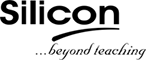
\includegraphics[scale=0.2]{figuras/SITWEST.png}
}
\subject{Whatever is on topic} % metadata

\graphicspath{{figuras/}}
% --------------------------------------------------- %
%                    Title + Schedule                 %
% --------------------------------------------------- %

\begin{document}

\begin{frame}
  \titlepage
\end{frame}

\begin{frame}{Index}
  \tableofcontents
\end{frame}

% --------------------------------------------------- %
%                      Presentation                   %
% --------------------------------------------------- %
\section{Restaurant Recommendation system based on location}
\begin{frame}{system}
	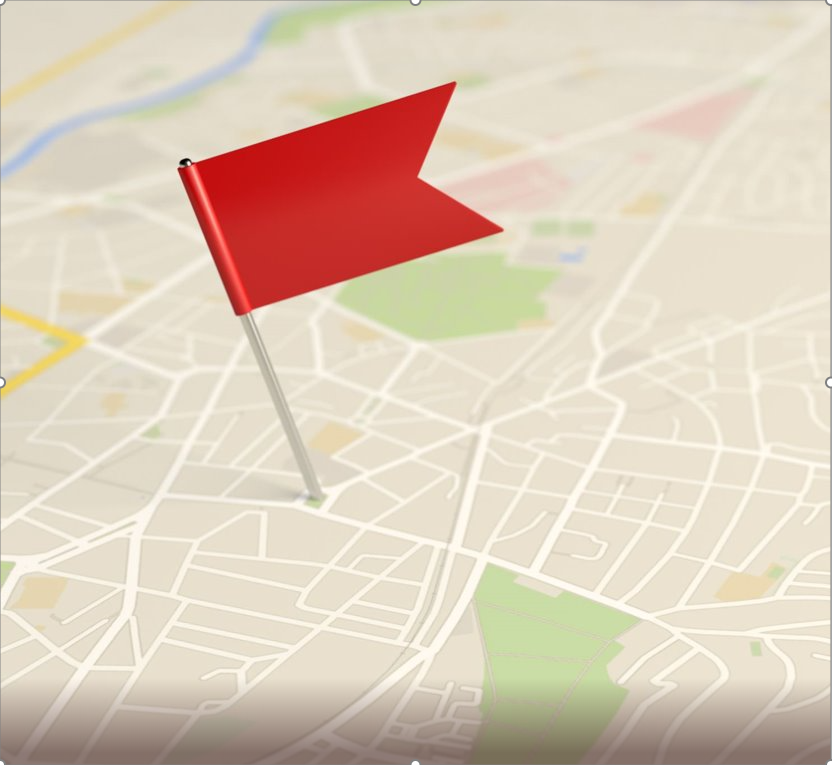
\includegraphics[scale=0.45]{figuras/pin.png}
	
\end{frame}
\section{Abstract}
\begin{frame}{Abstract}

\begin{columns}
\begin{column}{0.43\textwidth}
\centering

\includegraphics[scale=0.0065]{figuras/CART.png}
\boxorange{
\centering

\includegraphics[scale=0.7]{figuras/CART.png}
The Recommendation system is the unavoidable thing for whatever we buy or go to the new place.}
\end{column}

\begin{column}{0.43\textwidth}
\boxorange{
\centering

\includegraphics[scale=0.5]{figuras/Officer.png}
Restaurants also need recommendation systems in terms of attracting more customers in the management side and tasting favorite, famous food in the restaurant in customers side.}

\end{column}
\begin{column}{0.4\textwidth}
\boxorange{
\centering

\includegraphics[scale=0.8]{figuras/snack.png}
In reality finding the favorite food and famous food especially in new area is a challenging task.}

\end{column}

\begin{column}{0.4\textwidth}
\boxgrey{
\centering

\includegraphics[scale=0.5]{figuras/image.png}

Ranking scheme can be employed based on scores. The output of the model may be recommending most popular restaurants and most popular food items served by the appropriate restaurant}

\end{column}
\begin{column}{0.4\textwidth}
	\begin{itemize} 
		\item This autonomous 
		switching of the system between online and offline modes 
		guarantee that there is no wastage of power and bandwidth 
		when it is not required. 
		\item The user will be tracked through Web 2.0 technologies 
		 namely HTML5 and the data set will be retrieved 
		simultaneously from Foursquare. Based on the user’s checkin to any restaurant, the data will be added to the restaurant 
		data set and will then be evaluated for user interest profile. 
		This application will mostly be running in the background, 
		as participation from user is avoided as much as possible. 
	\end{itemize}
\end{column}
\end{columns}
	
\end{frame}

\section{Motivation}
\begin{frame}{Motivation}
	\begin{itemize}
		\item The motive of this paper is to present an implemented 
		design of the recommendation system. The system 
		architecture presented in Figure 1 can be simply divided into 
		two sections, one which has online activity, and the other 
		which processes data offline. When the user is in motion, 
		i.e., his geo-position changes notably, the system goes online 
		and recommendation module becomes active, retrieving 
		nearby and restaurants and ranking them, based on their 
		properties, according to the scores generated offline.
		\item  The offline part generally remains in a non-functional mode 
		when the user is stationary The work of the offline system is 
		to generate a user interest profile, using a Machine Learning 
		algorithm, from the data set that keeps getting modified 
		whenever the user checks-in a restaurant. 
		
	\end{itemize}
	\begin{center}
		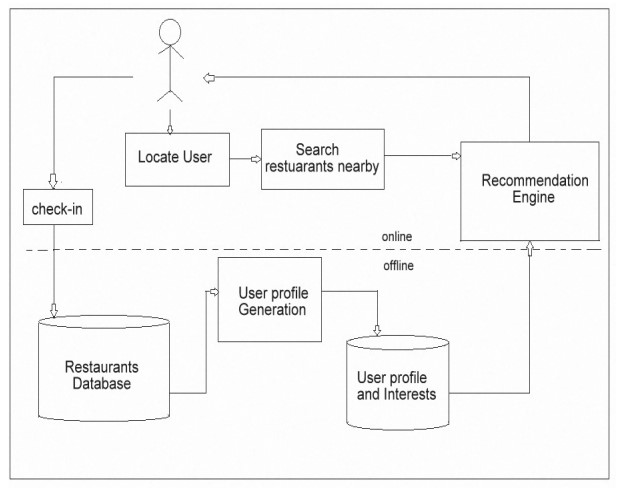
\includegraphics[scale=0.4]{Screenshot 2023-05-09 102947.jpg};
	\end{center}
\end{frame}

\begin{frame}
	\begin{itemize}
		\item This autonomous 
		switching of the system between online and offline modes 
		guarantee that there is no wastage of power and bandwidth 
		when it is not required. 
			\item Based on the type of functionalities , the system can 
		be divided into different modules, i.e., database layer, 
		recommendation engine, user profile generator and online 
		interaction layer. 
		\item The user will be tracked through Web 2.0 technologies 
		[9] namely HTML5 and the data set will be retrieved 
		simultaneously from Foursquare. Based on the user’s checkin to any restaurant, the data will be added to the restaurant 
		data set and will then be evaluated for user interest profile. 
		This application will mostly be running in the background, 
		as participation from user is avoided as much as possible. 
	\end{itemize}

\end{frame}
\section{Introduction}
\begin{frame}{Contents}
\begin{columns}
\begin{column}{0.25\textwidth}
\centering

\includegraphics[scale=0.5]{figuras/kimbo.png}
Overview
\end{column}

\begin{column}{0.25\textwidth}
\centering

\includegraphics[scale=0.5]{figuras/pc.png}
Working Principle

\end{column}

\begin{column}{0.25\textwidth}

\centering

\includegraphics[scale=0.5]{figuras/code.png}
Features

\end{column}
\begin{column}{0.25\textwidth}
\centering

\includegraphics[scale=0.5]{figuras/app.png}
Application

\end{column}
\end{columns}
\end{frame}
\begin{frame}{Overview}
	\begin{itemize}
		\item A recommendation system is a subclass of Information filtering Systems that seeks to predict the rating or the preference a user might give to an item. In simple words, it is an algorithm that suggests relevant items to users.
		\item  Restaurants also need recommendation systems in terms of attracting more customers in the management side and tasting favorite, famous food in the restaurant in customers side. In reality finding the favorite food and famous food especially in new area is a challenging task. By using this recommendation system for restaurants based on food rating distribution, service rating distribution by calculating the matrix density. With addition to that we build the popularity based recommender model for recommending restaurants to the customers. 
		\item Ranking scheme can be employed based on scores. The output of the model may be recommending most popular restaurants and most popular food items served by the appropriate restaurant. For betterment of the model we accompany collaborative filtering with singular value decomposition. Evaluation of the model can be completed with RMSE. This experiment is executed on the Kaggle data set and we build a web based application is built using python’s Flask web frame work.
	\end{itemize}
\end{frame}

\subsection{Overview}
\subsection{Working Principle}
\begin{frame}{Working principle }
	\begin{itemize}
		\item LEARNING USER PROFILE
		\item RECOMMENDATION ENGINE
		\item IMPLEMENTATION
	\end{itemize}
\end{frame}
\begin{frame}{LEARNING USER PROFILE}
	\begin{itemize}
		\item Restaurants are classified as ‘like’ or ‘dislike’, depending 
		on the taste of the user.
		\item Each 
		restaurant would account for n entries, where n is the number 
		of check-ins made. Further, if he likes two restaurants, which 
		one would he favor more? We solve this problem by using 
		Naïve Bayes Classifier algorithm to recognize the factors 
		that the user likes about a restaurant and to what degree does 
		he like them.
	\end{itemize}
	
	
\end{frame}
\begin{frame}{	Naïve Bayes}
	\begin{itemize}
		\item  Naïve Bayes algorithm is a supervised learning algorithm, which is based on Bayes theorem and used for solving classification problems
		\item Among the two formulations of Naïve Bayes, 
		we have found out that multinomial Bernoulli model would 
		be more efficient in this context, as its calculations are based 
		on word frequency information.
		\item The factors 
		that the user likes about a restaurant and to what degree does 
		he like them
	\end{itemize}

	\end{frame}
	
	\begin{frame}{RECOMMENDATION ENGINE}
	content...
	\end{frame}
	
	\begin{frame}{IMPLEMENTATION}
	content...
	\end{frame}
\subsection{Features}
\subsection{Application}


% --------------------------------------------------- %
%                      Presentation                   %
% --------------------------------------------------- %



\section{Conclusion}
\begin{frame}{Conclusion}

Normal text \alert{Alert Text}  \exemple{Example Text} \emph{Emphasis Text}
\begin{columns}

\begin{column}{0.5\textwidth}

\begin{block}{Simple block}
  \begin{itemize}
  	\item ...
  \end{itemize}
\end{block}

\begin{exampleblock}{Example block}
  \begin{itemize}
  	\item ...
  \end{itemize}
\end{exampleblock}

\begin{alertblock}{Alert block}
  \begin{itemize}
  	\item ...
  \end{itemize}
\end{alertblock}

\end{column}

\begin{column}{0.5\textwidth}

\boxpurple{
\centering
A purple box}

\boxorange{
\centering
An orange box}

\boxgrey{
\centering
A gray box}

\begin{tcolorbox}[tablegreen,tabularx={X||Y|Y|Y|Y||Y}, boxrule=0.5pt, title=My price table]
Color & Price 1  & Price 2  & Price 3 \\\hline\hline
Red   & 10.00   & 20.00   &  30.00 \\\hline
Green    & 20.00   & 30.00   &  40.00  \\\hline
Blue    & 30.00   & 40.00   &  50.00 \\\hline\hline
Orange  & 60.00   & 90.00   & 120.00 
\end{tcolorbox}

\end{column}

\end{columns}
\end{frame}


\section{References}
\begin{frame}{References}
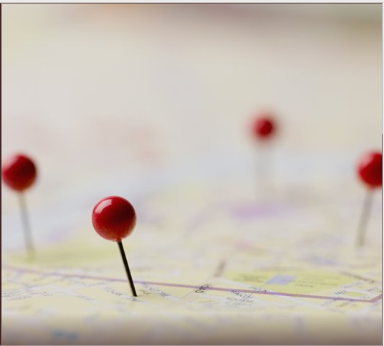
\includegraphics[scale=1]{figuras/pins.png}
    
\end{frame}

\end{document}
